\documentclass[11pt]{article}
\usepackage{mystyle}

\title{Notes on x-ray data bit-depth}
\author{Scott Trinkle}
\date{Last edited: \today}

\newsavebox{\largestimage}

\begin{document}

\maketitle

\section{Introduction}

The aim of these notes is to discuss and characterize the post-processing steps
involved in preparing the reconstructed $\upmu$CT data for further analysis.

\subsection{Data size reduction}
The full resolution (1.2 $\upmu$m isotropic) $\upmu$CT data\footnote{In these
  notes, I refer to what I am told is the ``best'' $\upmu$CT dataset that has a
  corresponding DW-MRI volume, located in
  \texttt{/data\char`_raf/2018\char`_04\char`_03\char`_WholeBrainMRI1\char`_retake\char`_newfocus/recon\char`_flatcorr\char`_1x/}
  on globus.}  is reconstructed with 32-bit float precision, with an image size
of 9168$\times$9168$\times$14521 voxels. A single slice is \textapprox 336 MB
and the full volume is \textapprox 4.8 TB. There are a number of post-processing
steps performed to reduce the data size. First, each slice is cropped to a
9156$\times$5958 voxel field of view that just includes the extent of the brain
volume. Next, the data are rescaled from 32-bit floating point values to
8-bit unsigned integers. These two operations reduce a single slice to \textapprox
52 MB, a reduction of \textapprox 85\%. A comparison of the pre- and
post-processed data with the corresponding gray-value histograms are shown in
Figure~\ref{fig:datacomp}.

\begin{figure}[h]
  \centering
  \savebox{\largestimage}{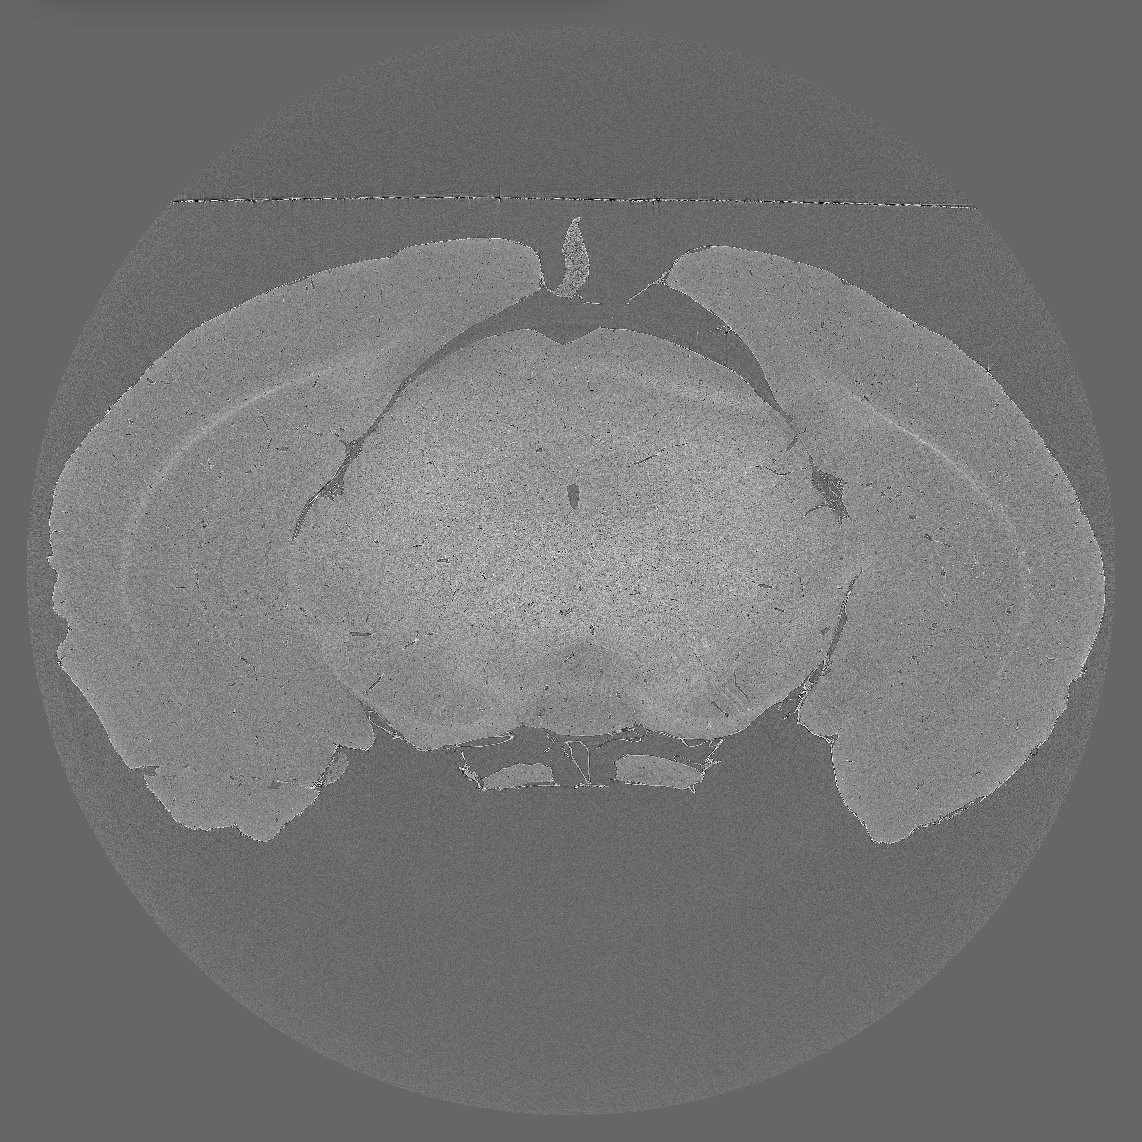
\includegraphics[width=0.432\linewidth]{figs/recon32}}
  \begin{subfigure}[t]{0.48\textwidth}
    \centering
    \usebox{\largestimage}
  \end{subfigure}
  \hspace{1em}
  \begin{subfigure}[t]{0.48\textwidth}
    \centering
    \raisebox{\dimexpr.5\ht\largestimage-.5\height}{%
      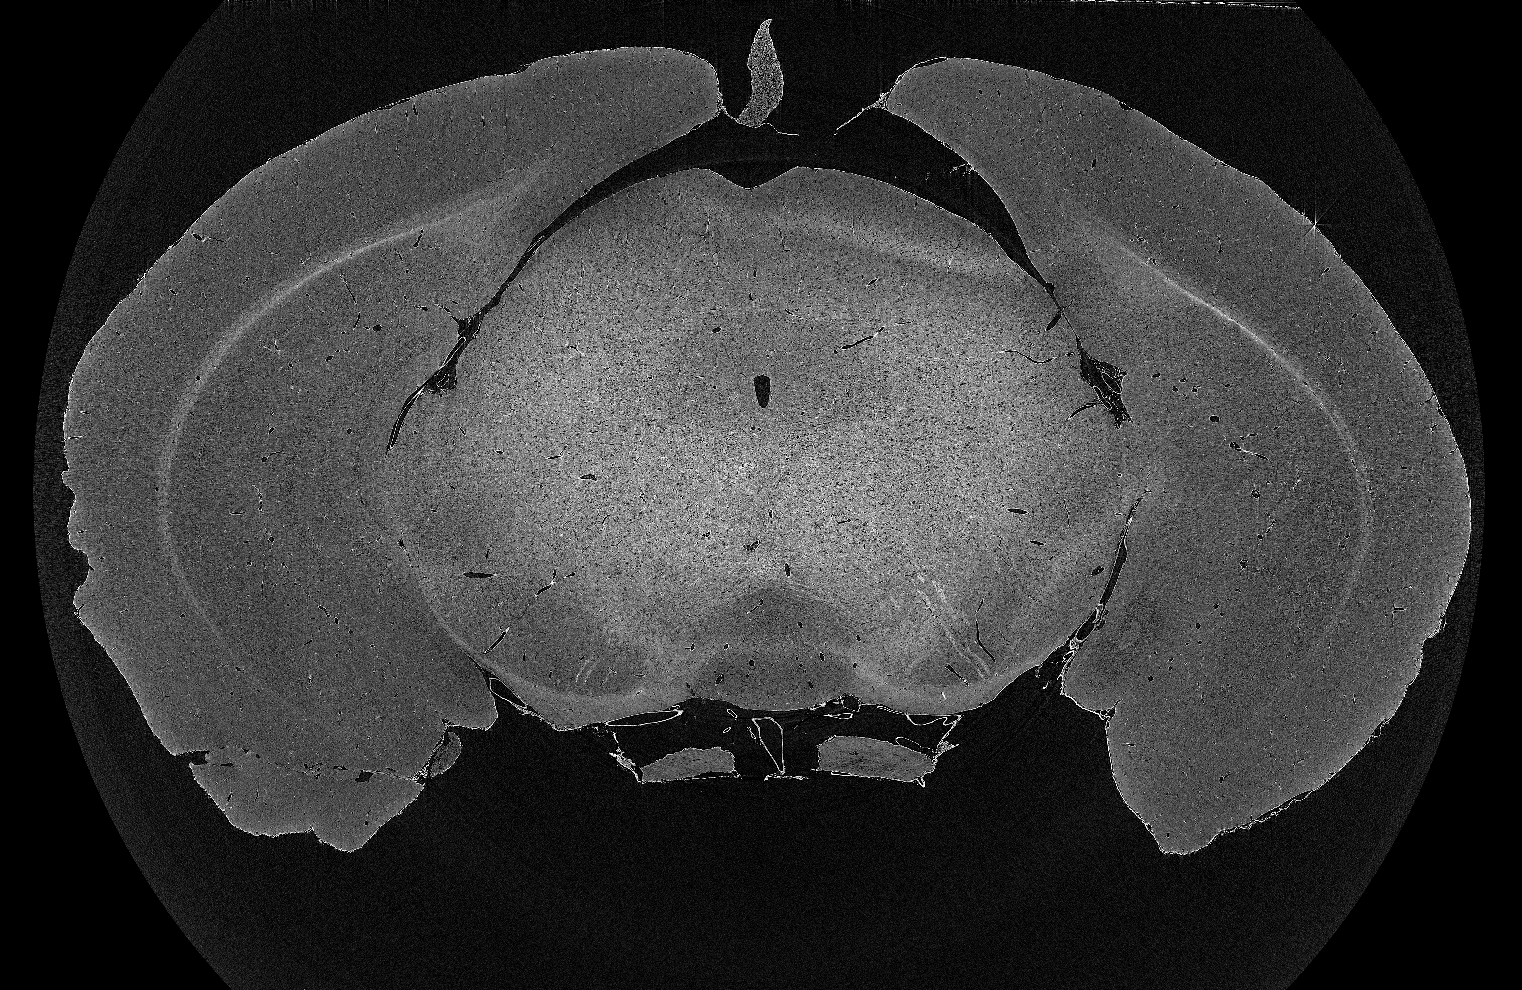
\includegraphics[width=0.9\linewidth]{figs/recon8}}
  \end{subfigure}
  \vspace{1em}
  \begin{subfigure}[b]{0.48\textwidth}
    \centering
    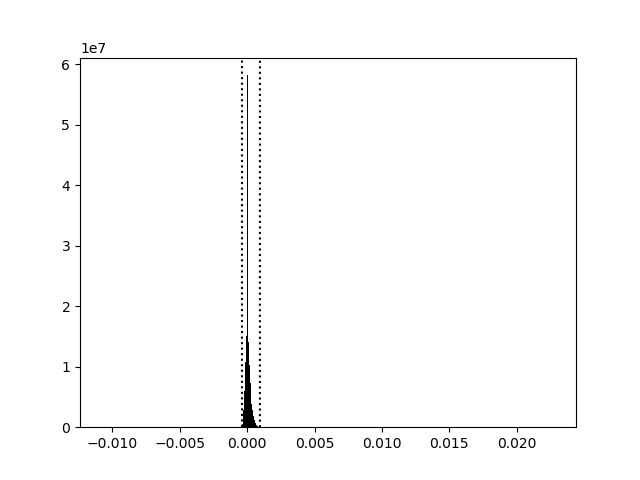
\includegraphics[width=0.9\linewidth]{figs/recon_orig_hist}
    \caption{Raw 32-bit slice. Display: [-6.68e-4, 0.001]}
  \end{subfigure}
  \hspace{1em}
  \begin{subfigure}[b]{0.48\textwidth}
    \centering
    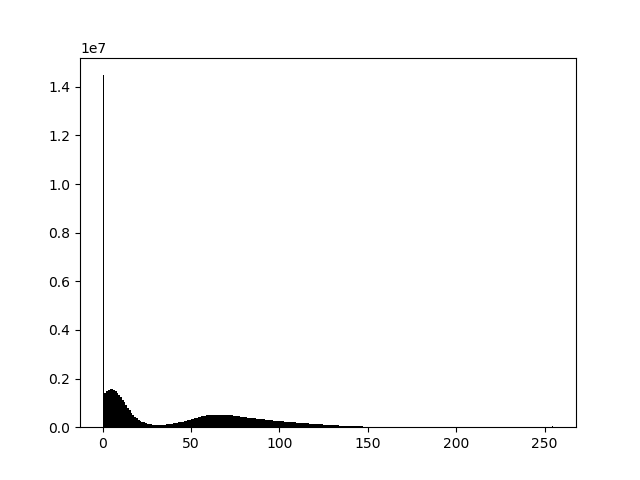
\includegraphics[width=0.9\linewidth]{figs/recon_crop8_hist}
    \caption{Cropped, 8-bit, rescaled slice}
  \end{subfigure}
  \caption{Comparison of raw and processed reconstructed data. (Note that the
    dotted lines represent the display range, not the rescaling thresholds.}
  \label{fig:datacomp}
\end{figure}

\subsection{Rescaling method}
Rescaling of the existing whole-brain datasets has been performed by Raf Vescovi
in ImageJ.  The global histogram is calculated and voxel values between some
\texttt{display\char`_min} and \texttt{display\char`_max} are scaled to values
between 0-255 and recast as 8-bit unsigned integers. To my knowledge, there is
not an established, reproducible method used to choose these scaling thresholds,
it is at the user's discretion. There also does not seem to be any documentation
detailing the choice of these thresholds for datasets which have already been
rescaled --- Raf claims to generally use \texttt{display\char`_min} = 0.0 and
\texttt{display\char`_max} $\approx$ 0.0015.

\section{Quantifiyng the rescaling effect on FODs}
The reduction in data size from casting 32-bit float values to 8-bit integers
necessarily comes at the cost of a loss of information. From qualitative visual
inspection, it appears that the rescaling process primarily discards
\textit{non-useful} information --- the rescaled image appears to be less noisy
and have higher contrast, particularly for white matter. For our purposes, the
effect of this process can be quantified by comparing the FODs calculated from
each of the two datasets using structure tensor analysis.

\subsection{Methods}
\subsection{Crop}
The raw 32-bit and reswcaled, cropped 8-bit datasets were downloaded from
globus. Raf did not provide the pixel locations used to crop the dataset, so
these were estimated using the location of common landmarks within matching
slices from the two volumes.  Figure~\ref{fig:composite} shows a composite image
of Raf's crop (red) with my attempt to match it (green). I estimate that my crop
matches his reasonably well, certainly within a few voxels.


\begin{figure}[h]
  \centering
  \begin{subfigure}[b]{0.48\textwidth}
    \centering
    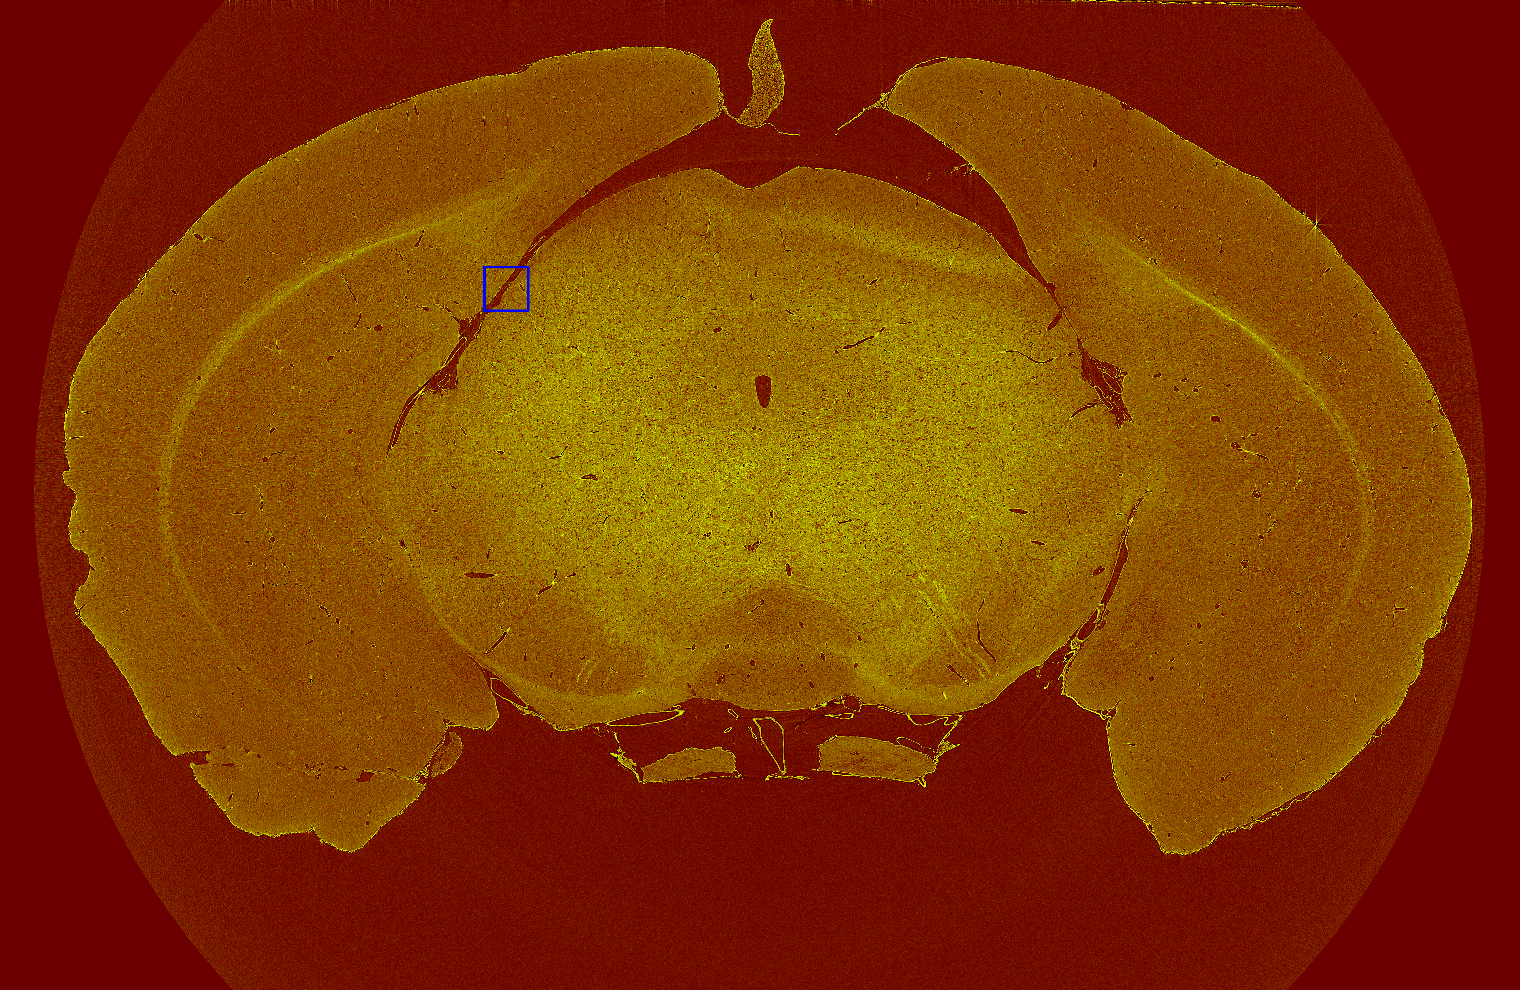
\includegraphics[height=5cm]{figs/composite_labeled}    
  \end{subfigure}
  \hspace{1em}
  \begin{subfigure}[b]{0.48\textwidth}
    \centering
    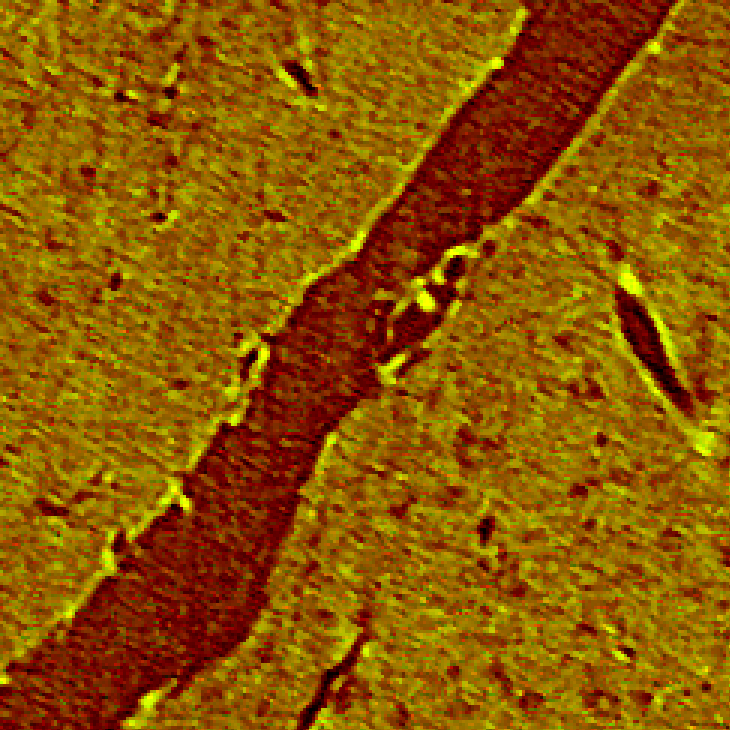
\includegraphics[height=5cm]{figs/composite_insert}    
  \end{subfigure}
  \captionsetup{width=0.9\textwidth}
  \caption{Composite of my crop (green) with Raf's crop (red). From visual
    inspection, there seems to be agreement within a few voxels at most.}
  \label{fig:composite}
\end{figure}

\subsection{Sample selection and FOD calculation}
A brain region was chosen with easily identifiable white matter tracts. FODs
were calculated from a uniform 15$\times$15 grid of MRI-voxel-sized
(125$\times$125$\times$125) ROI within both 32-bit and 8-bit brain volumes, for
a total of 225 FODs each. For this study, FODs were not thresholded by the
structure tensor fractional anisotropy value. The FODs were saved as a list of
spherical harmonic coefficients up to $L_{max}=20$.

\subsection{Comparison}
FODs calculated from the same region in the 32-bit and 8-bit datasets were
compared using a number of comparison metrics. The angular correlation
coefficient (ACC) effectively reports the correlation between spherical harmonic
coefficients. The Jenson-Shannon divergence (JSD) measures the distance between
two probability distributions on the sphere. This was calculated by expanding
the spherical harmonic representation of each FOD onto a sphere with 1200
sampling points chosen with the Fibonacci algorithm. Finally, the root mean
squared error was calculated directly from the spherical harmonic
coefficients. Each of these metrics is detailed
\href{https://github.com/scott-trinkle/uCTdMRI/blob/master/notes/2018-05-22-tuning-parameters/report/report.pdf}{in
  an earlier report}.\

\subsubsection{Results}

Figure \ref{fig:histograms} shows the distributions of the three comparison
metrics for the 225 ROI. Overall, there is a relatively wide distribution in all
three metrics, meaning there is a high variability in the effect of data rescaling
on the FOD. Figure \ref{fig:scatter} shows scatterplots between pairs of metrics,
with corresponding correlation coefficients. Generally, these metrics show similar
trends and communicate similar information. 

\begin{figure}[h]
  \centering
  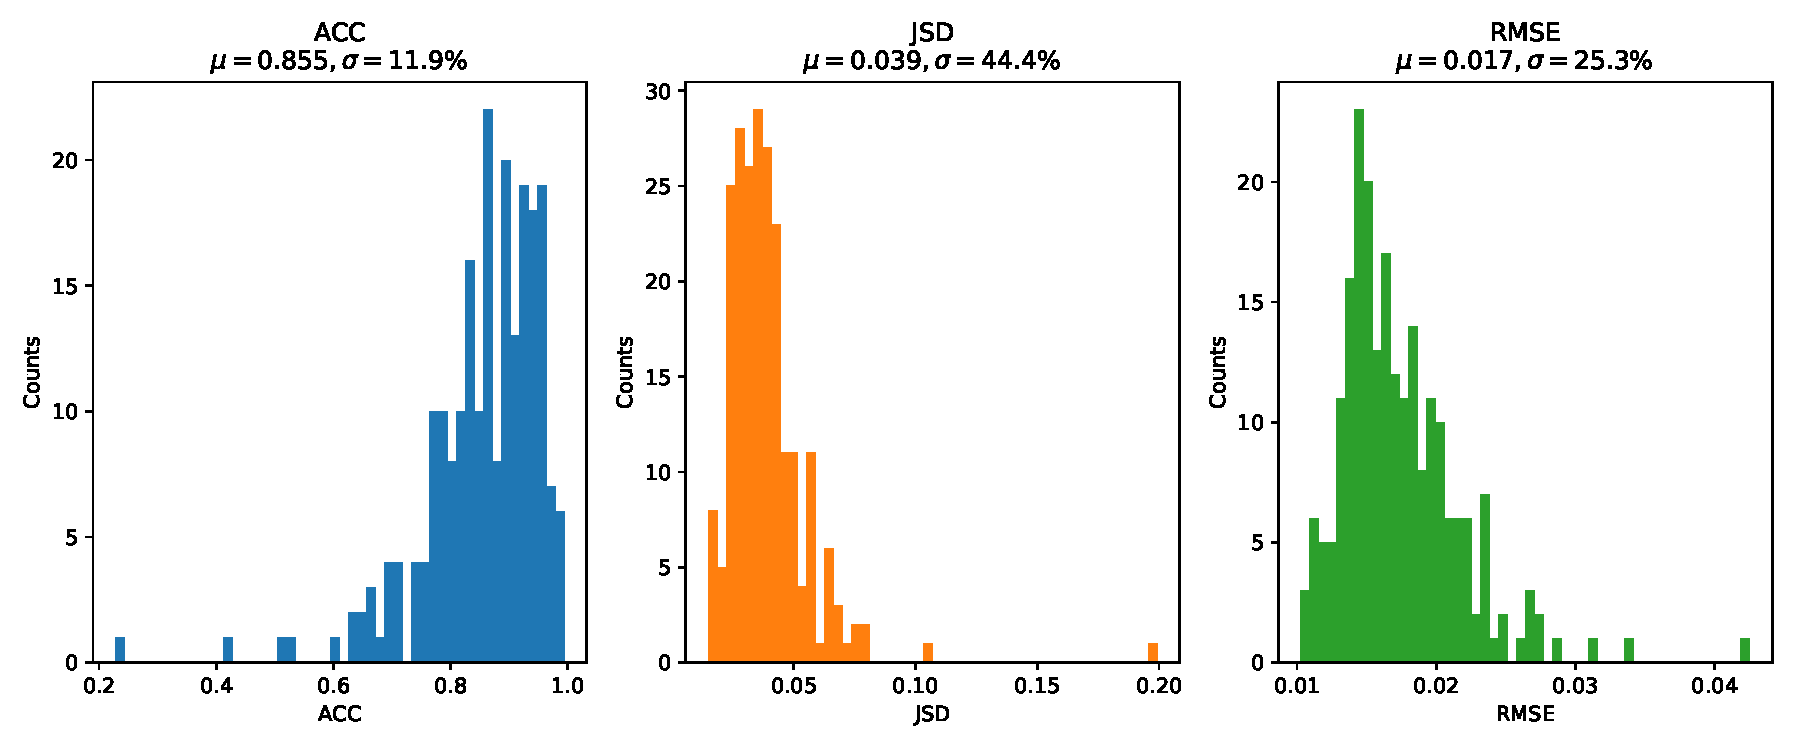
\includegraphics[width=0.95\textwidth]{../plots/hists}
  \caption{Comparison metric distributions}
  \label{fig:histograms}
\end{figure}

\begin{figure}[h]
  \centering
  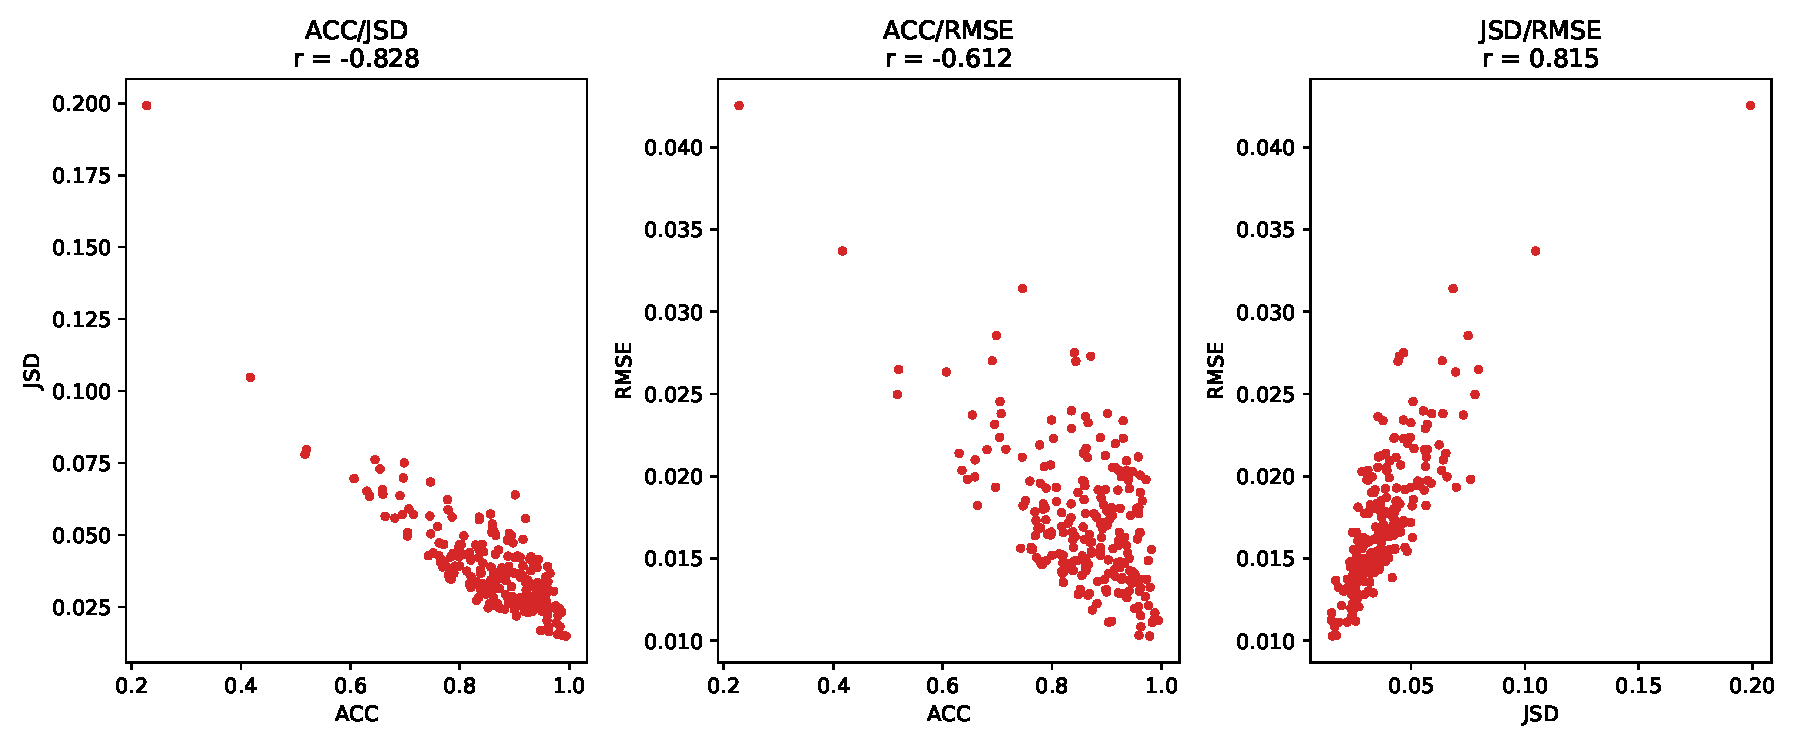
\includegraphics[width=0.95\textwidth]{../plots/scatter}
  \caption{Scatterplots of pairs of metrics. Generally, these three metrics seem
    to communicate similar information.}
  \label{fig:scatter}
\end{figure}

I was curious if there was a relationship between the shape of the FOD and
effect from rescaling --- i.e., whether there would be less of a deviation
between the 8-bit and 32-bit FODs for sharply oriented, single-peak FODs, as
opposed to more complex, multi-peak, arbitrary shaped FODs. This was tested by
calculating the generalized fractional anisotropy (GFA) of the FODs using the
\href{http://nipy.org/dipy/reference/dipy.reconst.html#gfa}{\texttt{gfa}}
function in the Dipy python package. The GFA is a metric from 0 to 1 that
quantifies the anisotropy of a function on the sphere.

Overall, this test was inconclusive. Figure \ref{fig:gfa} shows the GFA values
calculated from the 8-bit data plotted against the three comparison
metrics. There is a relatively weak linear relationship between GFA and ACC (r =
0.63), but a negligible relationship between GFA and the other two metrics.

\begin{figure}[h]
  \centering
  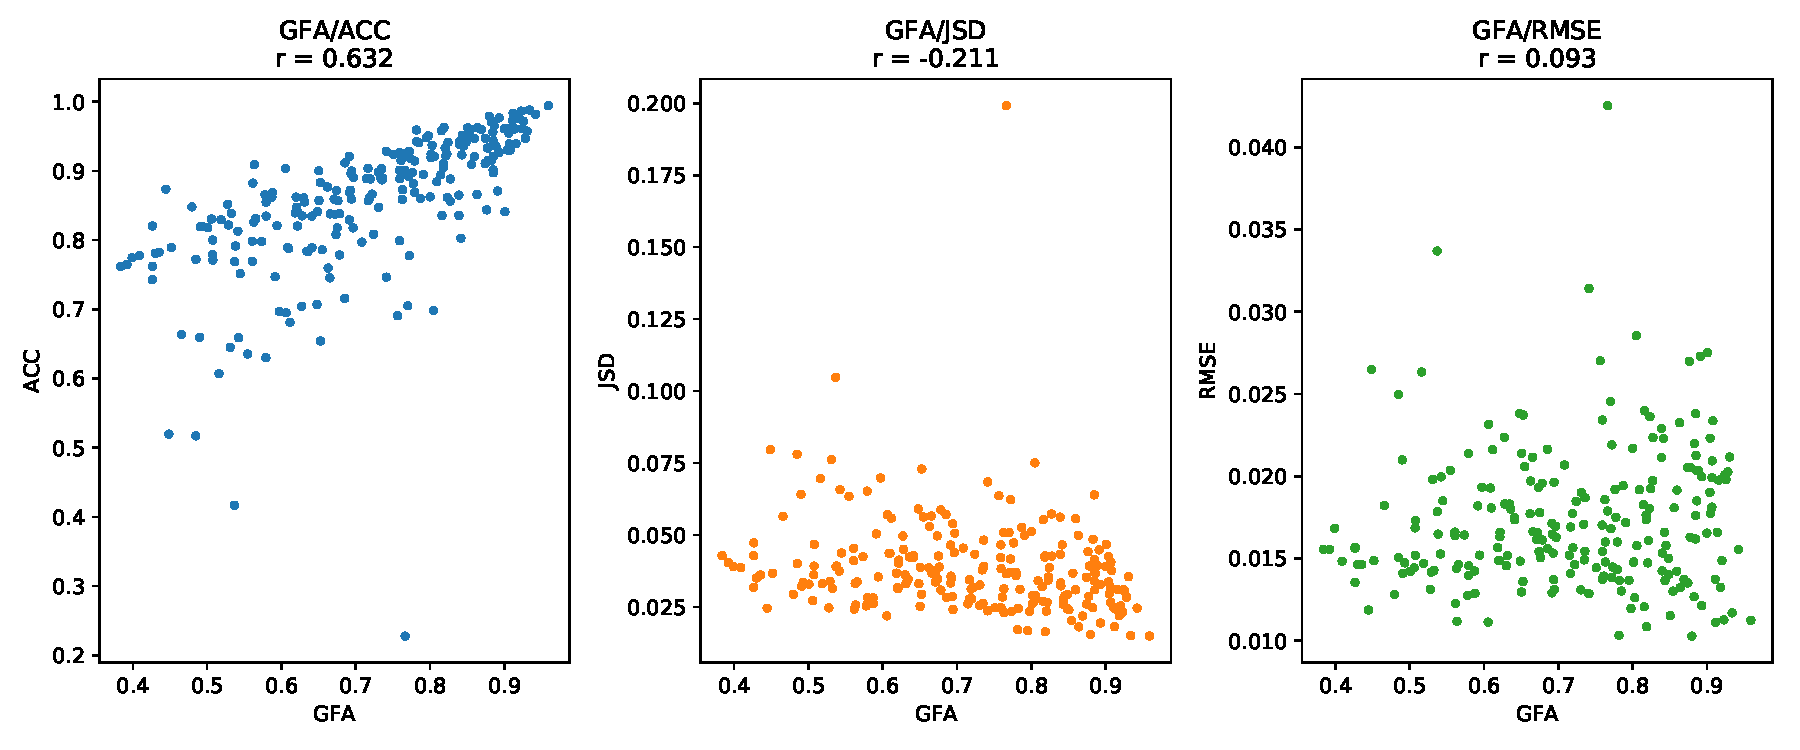
\includegraphics[width=0.95\textwidth]{../plots/gfa}
  \caption{GFA Scatterplots}
  \label{fig:gfa}
\end{figure}

I also thought it would be relavant to see the comparison metrics plotted as a
function of location in the data --- i.e., would FODs in prominent white matter
tracts show less of a deviation between scaled and unscaled datasets. Figure
\ref{fig:accmap} is an HSV (hue, saturation, value) image highlighting the test
ROI. The hue corresponds to the ACC, the saturation was constant for all ROI,
and the value corresponds to the 8-bit image data. From visual inspection, it
does seem that areas with lower ACC (blue, green, teal, etc.) tend to be located
in regions without much white matter. Similar images were calculated for the
other three metrics and are shown in Figures~\ref{fig:jsdmap}-\ref{fig:rmsemap}.

\begin{figure}[h]
  \centering
  \hspace{-5em}
  \begin{subfigure}[b]{0.9\textwidth}
    \centering
    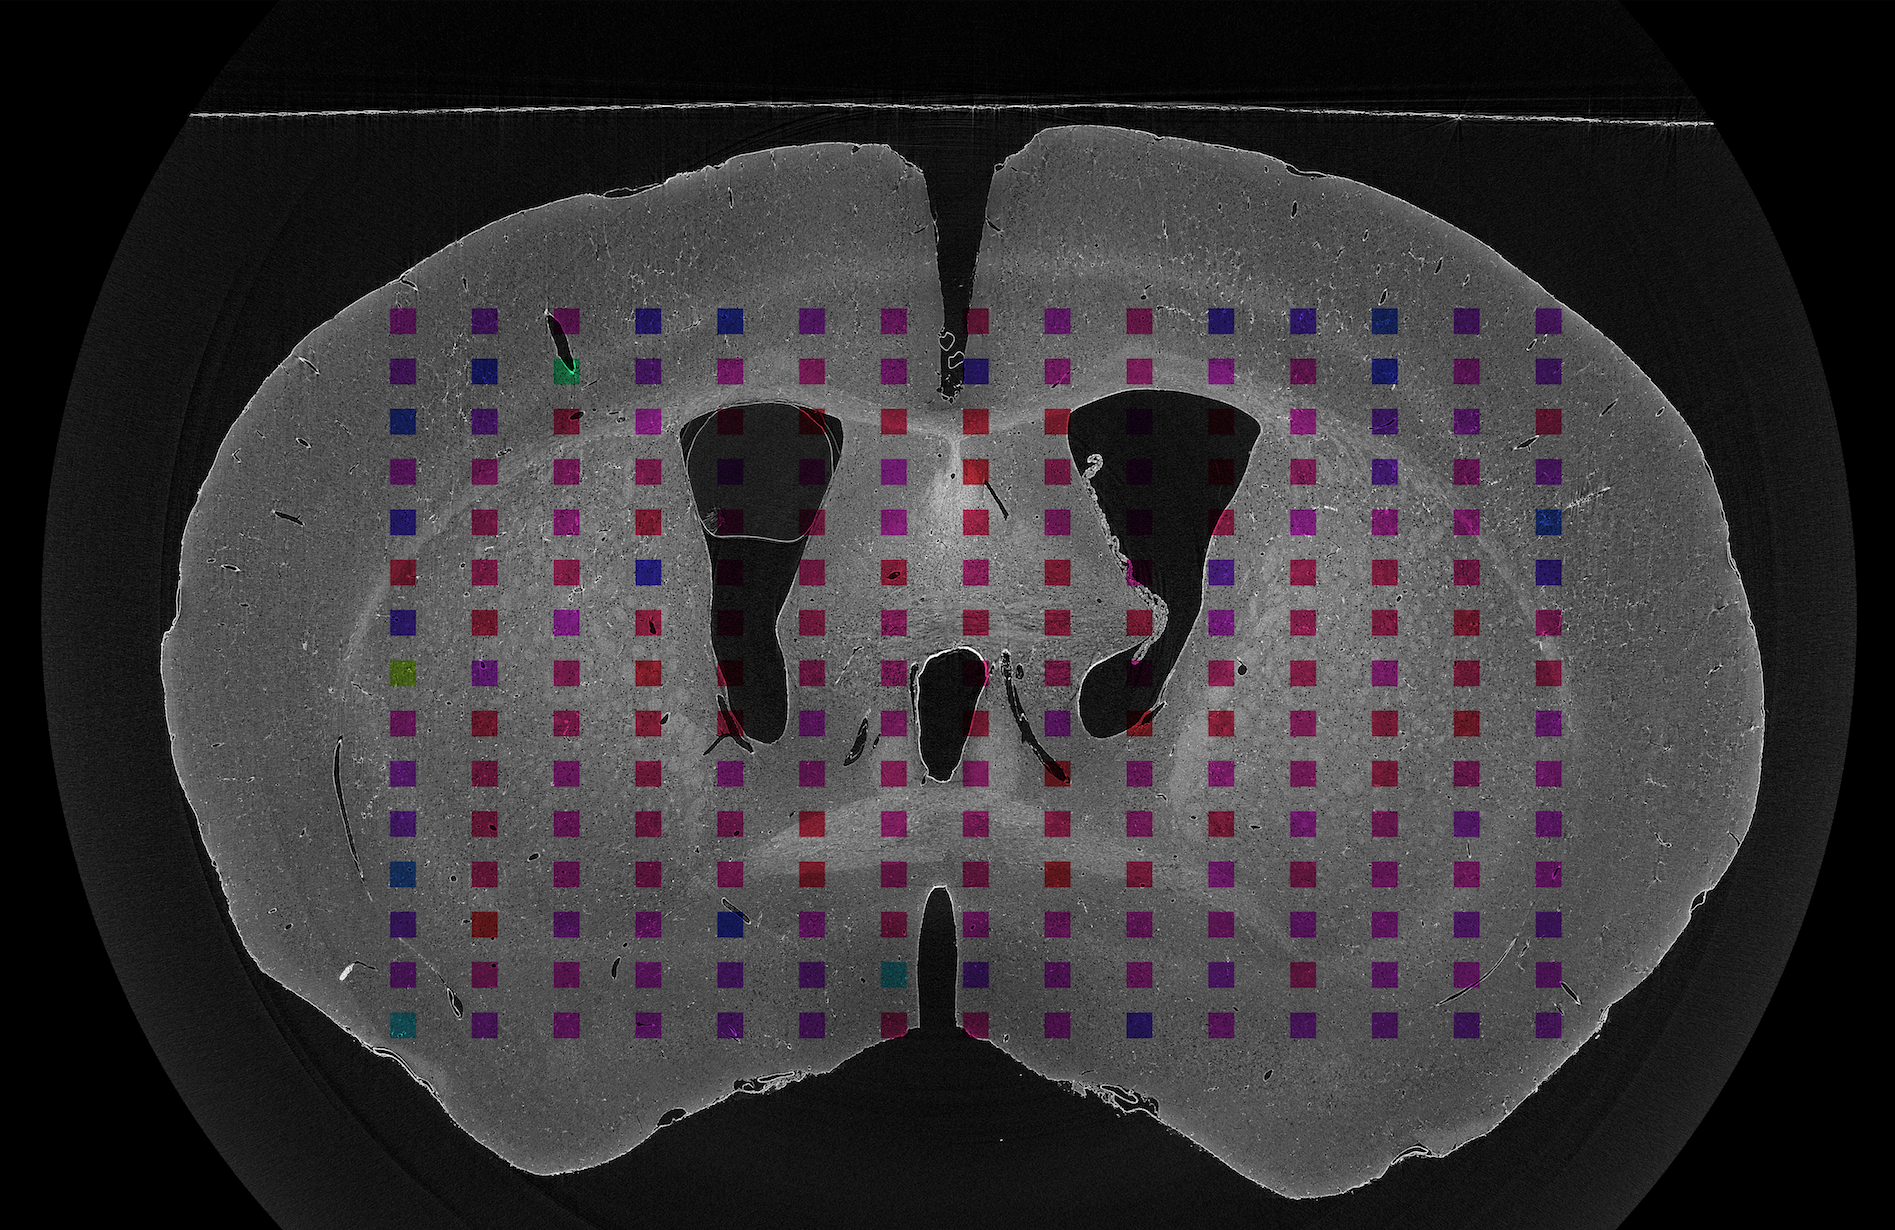
\includegraphics[height=9cm]{figs/acc}
  \end{subfigure}
  \hspace{-3em}
  \begin{subfigure}[b]{0.05\textwidth}
    \centering
    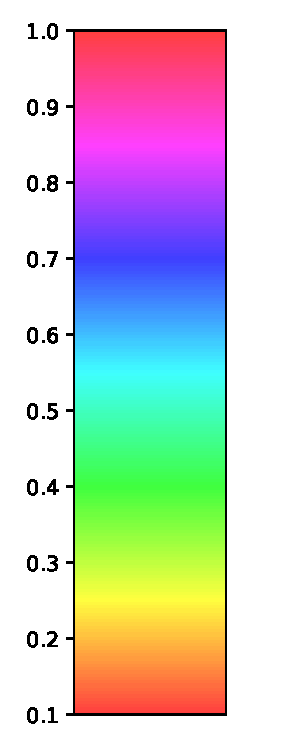
\includegraphics[height=9.1cm]{figs/cmap}
  \end{subfigure}
  \captionsetup{width=0.9\textwidth}
  \caption{ACC map}
  \label{fig:accmap}
\end{figure}

\begin{figure}[H]
  \centering
  \hspace{-5em}
  \begin{subfigure}[b]{0.9\textwidth}
    \centering
    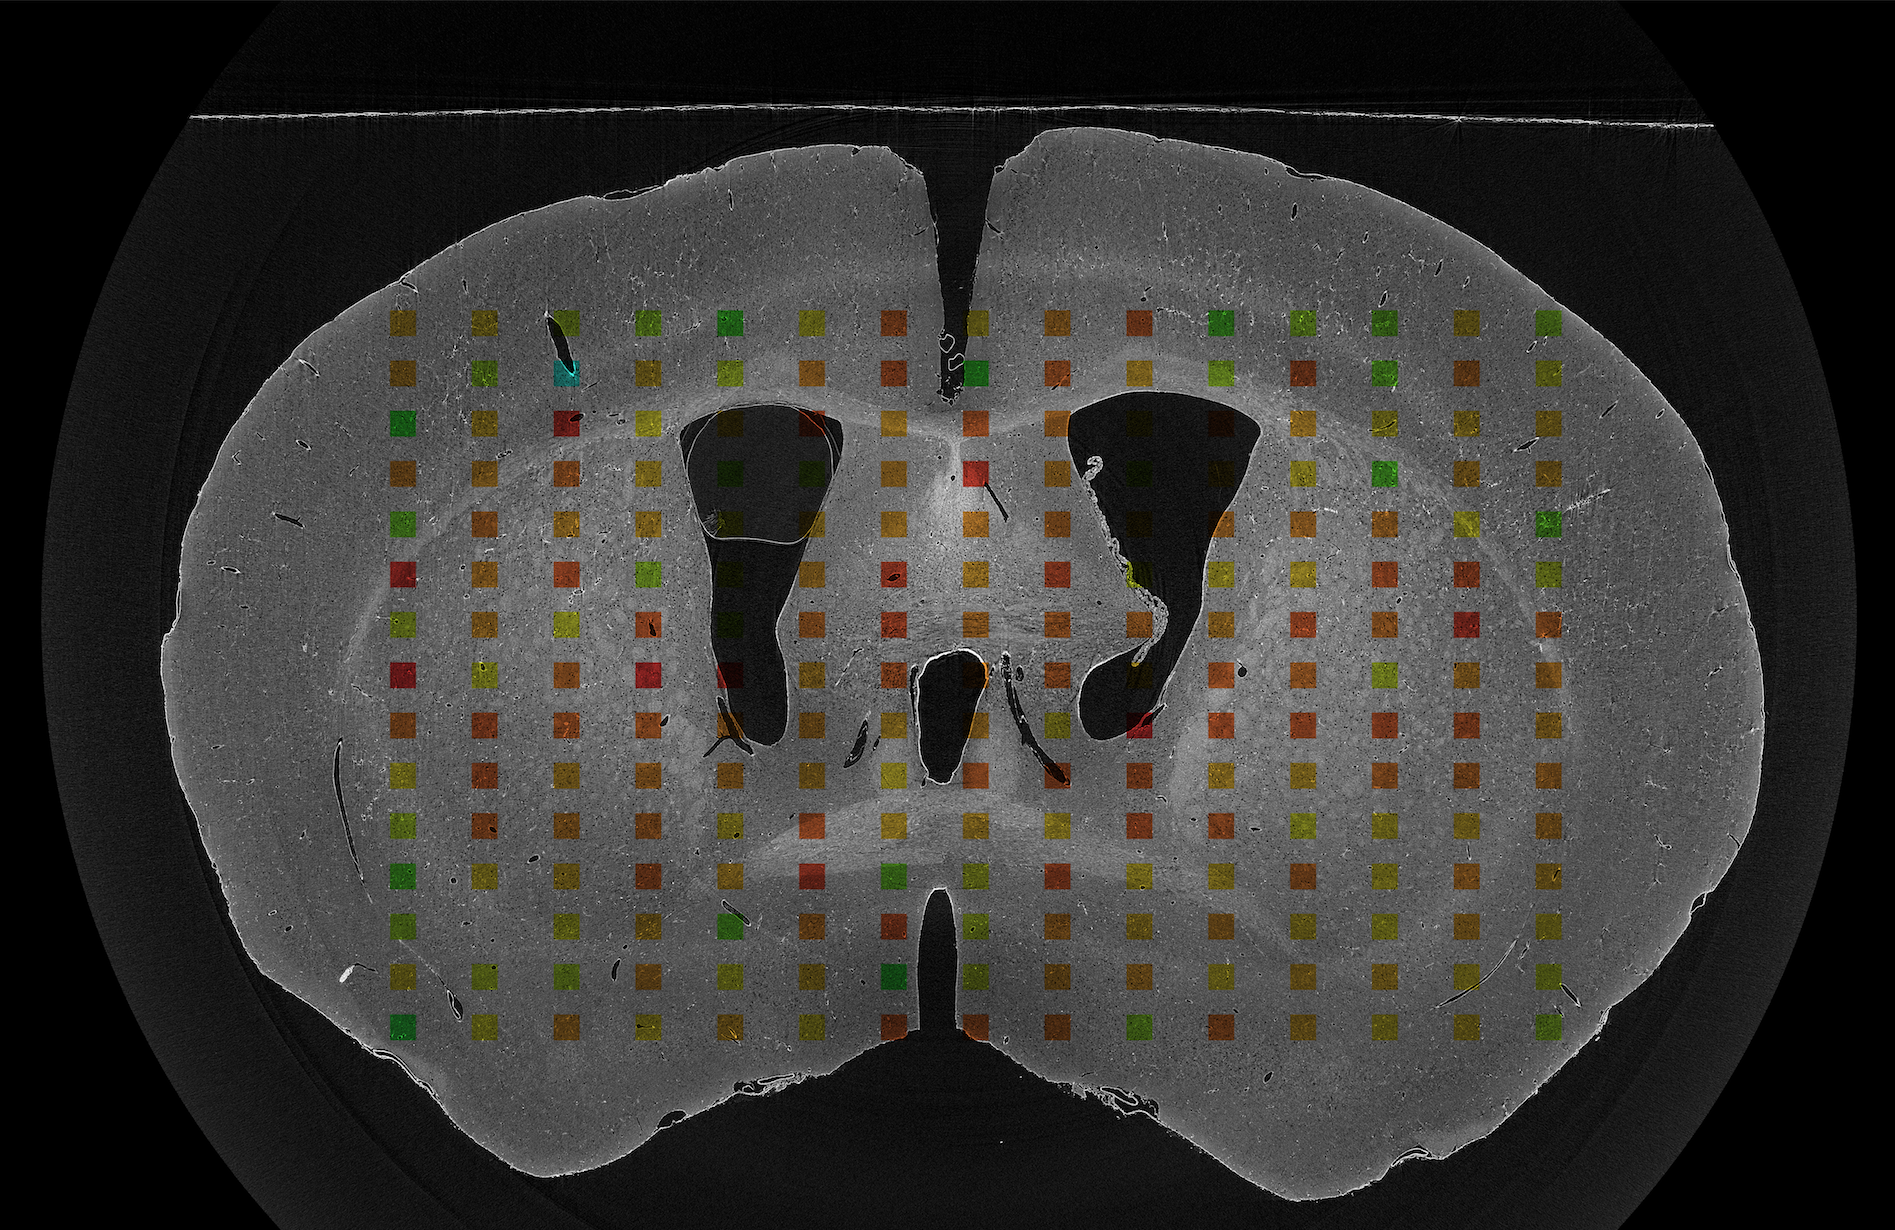
\includegraphics[height=9cm]{figs/jsd}
  \end{subfigure}
  \hspace{-3em}
  \begin{subfigure}[b]{0.05\textwidth}
    \centering
    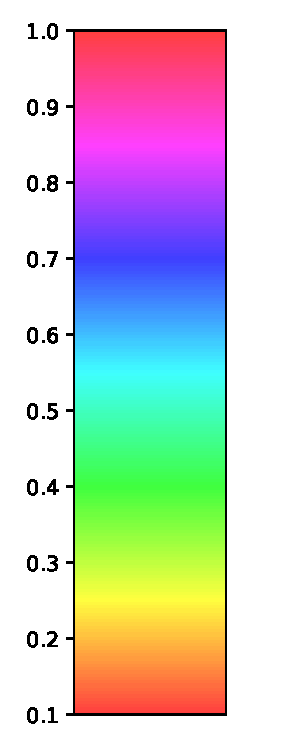
\includegraphics[height=9.1cm]{figs/cmap}
  \end{subfigure}
  \captionsetup{width=0.9\textwidth}
  \caption{JSD map (Values were normalized from 0-1 for visualization)}
  \label{fig:jsdmap}
\end{figure}

\begin{figure}[H]
  \centering
  \hspace{-5em}
  \begin{subfigure}[b]{0.9\textwidth}
    \centering
    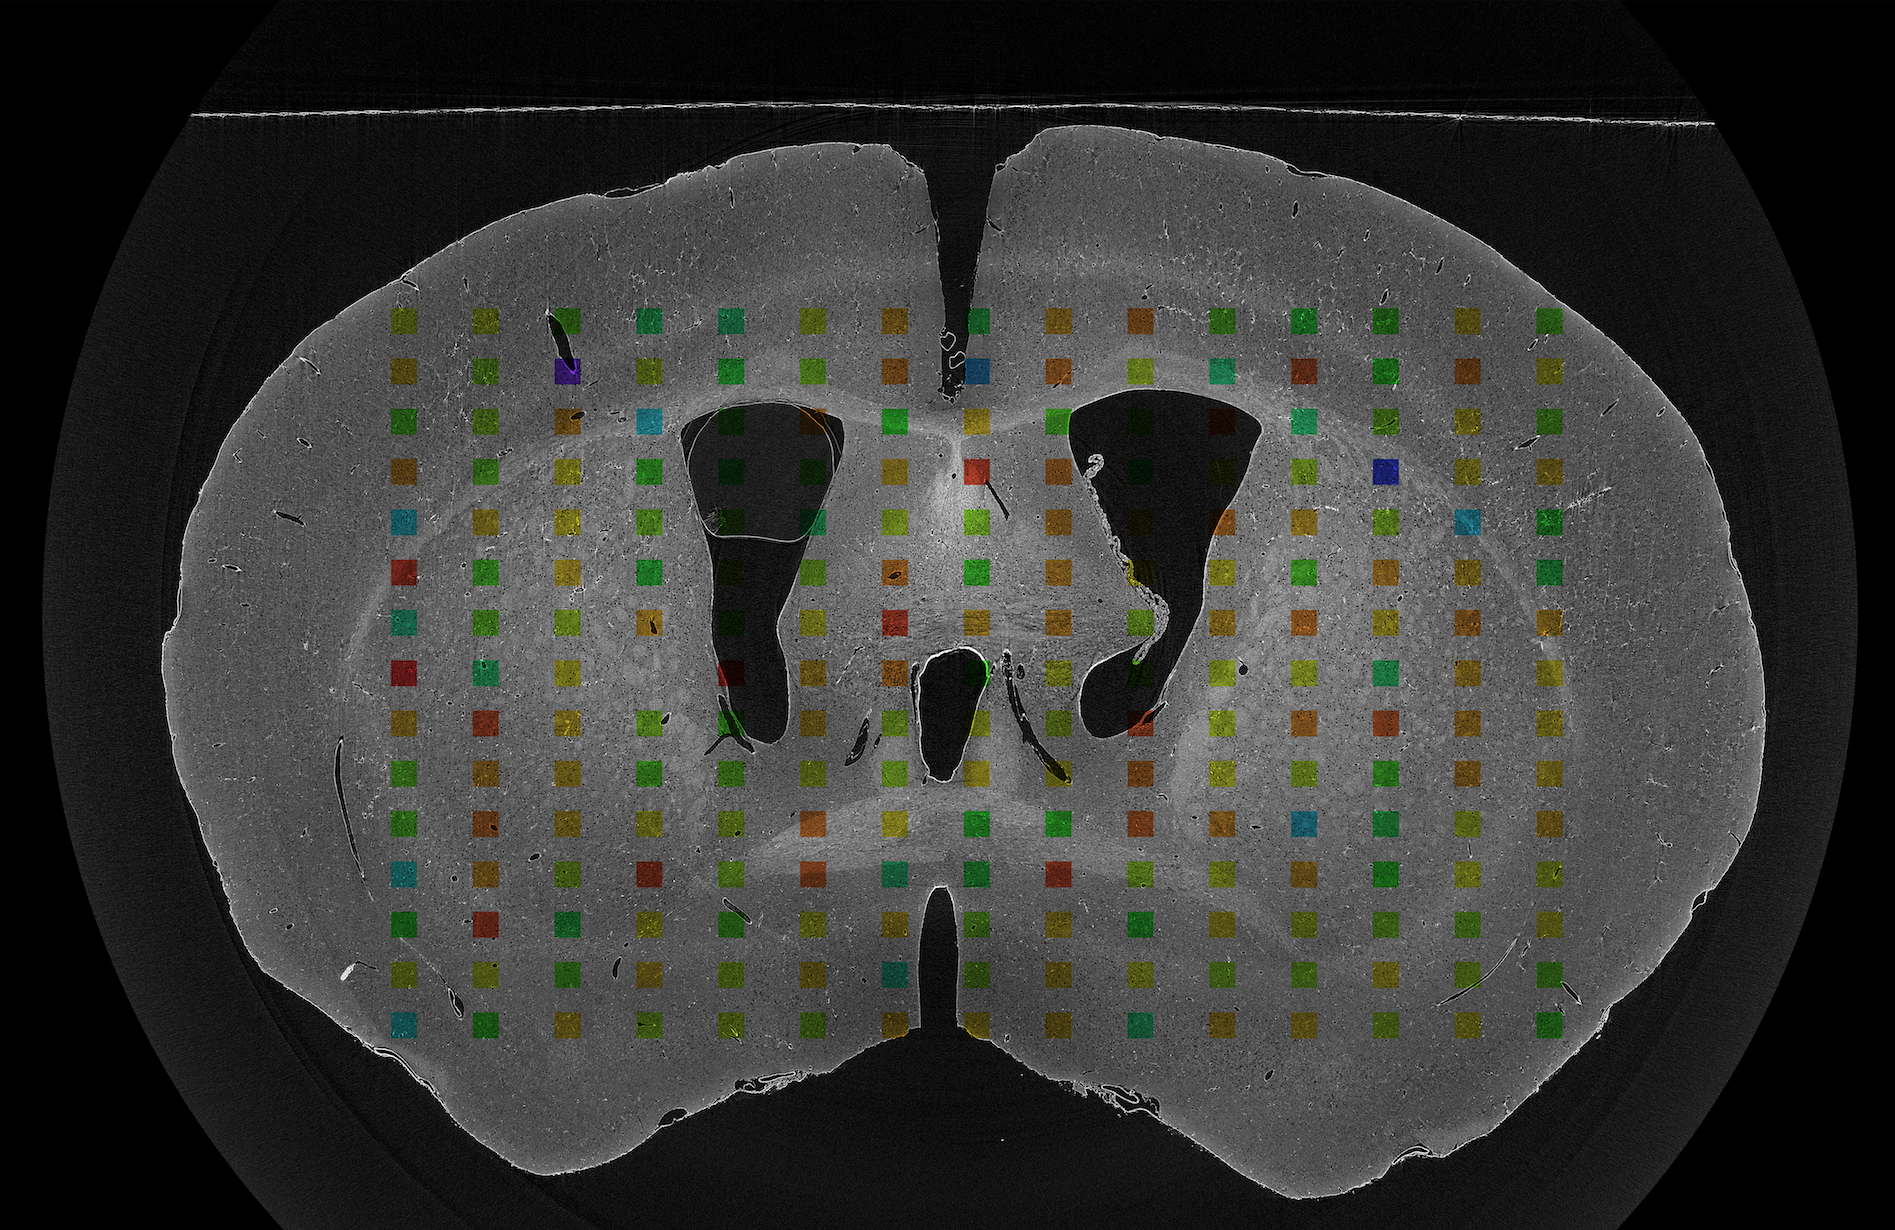
\includegraphics[height=9cm]{figs/rmse}
  \end{subfigure}
  \hspace{-3em}
  \begin{subfigure}[b]{0.05\textwidth}
    \centering
    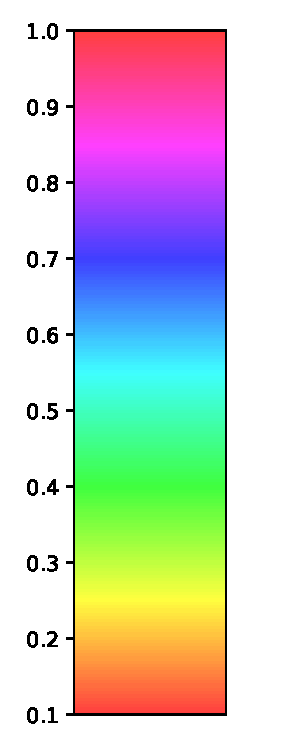
\includegraphics[height=9.1cm]{figs/cmap}
  \end{subfigure}
  \captionsetup{width=0.9\textwidth}
  \caption{RMSE map (Values were normalized from 0-1 for visualization)}
  \label{fig:rmsemap}
\end{figure}

Figure~\ref{fig:accs} is a visual demonstration of the discrepancy
in FOD shape as a function of ACC. 

% ACC, ID
% 0.23, 8
% 0.42, 32
% 0.52, 104
% 0.61, 12
% 0.70, 216
% 0.80, 198
% 0.90, 136
% 0.99, 28


\begin{center}
  \captionsetup{width=0.9\textwidth}
  \captionof{figure}{Caption}
  \begin{longtable}{M{0.15\textwidth} M{0.3\textwidth} M{0.3\textwidth}}
    ACC & 32-bit FOD & 8-bit FOD\\
     0.2 & \im{0.3}{\odfpath{32}{8}} & \im{0.3}{\odfpath{8}{8}}\\
     0.4 & \im{0.3}{\odfpath{32}{32}} & \im{0.3}{\odfpath{8}{32}}\\
     0.5 & \im{0.3}{\odfpath{32}{104}} & \im{0.3}{\odfpath{8}{104}}\\
     0.6 & \im{0.3}{\odfpath{32}{12}} & \im{0.3}{\odfpath{8}{12}}\\
     0.7 & \im{0.3}{\odfpath{32}{216}} & \im{0.3}{\odfpath{8}{216}}\\
     0.8 & \im{0.3}{\odfpath{32}{198}} & \im{0.3}{\odfpath{8}{198}}\\
     0.9 & \im{0.3}{\odfpath{32}{136}} & \im{0.3}{\odfpath{8}{136}}\\
     1.0 & \im{0.3}{\odfpath{32}{28}} & \im{0.3}{\odfpath{8}{28}}\\
   \end{longtable}
   \label{fig:accs}
\end{center}

\section{Conclusion}
The rescaling and conversion to 8-bit can clearly have a strong effect on the
overall FOD shape. More work is needed to understand the optimal pre-processing
steps needed to reduce the data size for efficient processing as well as to
understand the meaningful information in the noise.

However, the current implementation of the code already converts the data to
32-bit floating point values before beginning the FOD calculation pipeline.
With this in mind, the reduction in data size might only be relevant for storage
purposes, which is not a major issue --- data storage is cheap.

\end{document}
